
\iffalse
    \title{Assignment}
    \author{EE24BTECH11034}
    \section{ce}
    \chapter{2023}
  \fi
\item Which one of the following welding methods provides the highest heat flux $\brak{\frac{W}{mm}^2}$?

\begin{enumerate}
    \item Oxy-acetylene gas welding
    \item Tungsten inert gas welding
    \item Plasma arc welding
    \item Laser beam welding
\end{enumerate}

\item The length, width, and thickness of a steel sample are $400$ mm, $40$ mm, and $20$ mm, respectively. Its thickness needs to be uniformly reduced by $2$ mm in a single pass by using horizontal slab milling. The milling cutter $\brak{\text{diameter: } 100 \text{ mm}, \text{ width: } 50 \text{ mm}}$ has $20$ teeth and rotates at $1200$ rpm. The feed per tooth is $0.05$ mm. The feed direction is along the length of the sample. If the over-travel distance is the same as the approach distance, the approach distance and time taken to complete the required machining task are:

\begin{enumerate}
    \item $14$ mm, $18.4$ s
    \item $21$ mm, $28.9$ s
    \item $21$ mm, $39.4$ s
    \item $14$ mm, $21.4$ s
\end{enumerate}

\item The position vector $\overrightarrow{OP}$ of point $P \brak{20, 10}$ is rotated anti-clockwise in the $X-Y$ plane by an angle $\theta = 30^\circ$ such that point $P$ occupies position $Q$, as shown in the figure. The coordinates $\brak{x, y}$ of $Q$ are

\begin{center}
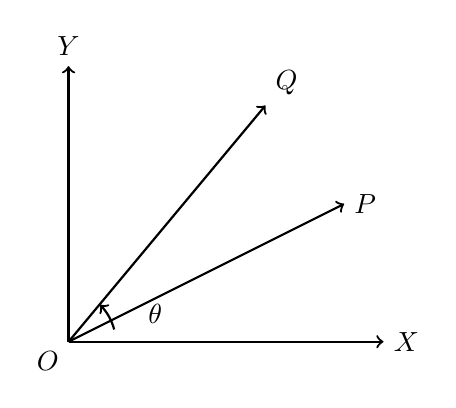
\begin{tikzpicture}
    \draw[->, thick] (0, 0) -- (4, 0) node[right] {$X$};
    \draw[->, thick] (0, 0) -- (0, 3.5) node[above] {$Y$};
    \draw[->, thick] (0, 0) -- (3.5, 1.75) node[right] {$P$};
    \draw[->, thick] (0, 0) -- (2.5, 3) node[above right] {$Q$};
    \draw[thick, ->, rotate=15] (0.6, 0) arc[start angle=0, end angle=30, radius=0.7];
    \node at (1.1, 0.35) {$\theta$};
    \node at (0, 0) [below left] {$O$};
\end{tikzpicture}
\end{center}

\begin{enumerate}
    \item $\brak{13.40, 22.32}$
    \item $\brak{22.32, 8.26}$
    \item $\brak{12.32, 18.66}$
    \item $\brak{18.66, 12.32}$
\end{enumerate}

\item The table presents the demand of a product. By simple three-months moving average method, the demand-forecast of the product for the month of September is

\begin{center}
\begin{tabular}{|c|c|}
\hline
\textbf{Month} & \textbf{Demand} \\
\hline
January & $450$ \\
February & $440$ \\
March & $460$ \\
April & $510$ \\
May & $520$ \\
June & $495$ \\
July & $475$ \\
August & $560$ \\
\hline
\end{tabular}
\end{center}

\begin{enumerate}
    \item $490$
    \item $510$
    \item $530$
    \item $536.67$
\end{enumerate}

\item Evaluation of $\int_{2}^{4} x^3 \, dx$ using a $2$-equal-segment trapezoidal rule gives a value of .

\item A cylindrical rod of diameter $10$ mm and length $1.0$ m is fixed at one end. The other end is twisted by an angle of $10^\circ$ by applying a torque. If the maximum shear strain in the rod is $p \times 10^{-3}$, then $p$ is equal to .
    
\item A solid cube of side $1$ m is kept at a room temperature of $32^\circ$C. The coefficient of linear thermal expansion of the cube material is $1 \times 10^{-5} $ and the bulk modulus is $200$ GPa. If the cube is constrained all around and heated uniformly to $42^\circ$C, then the magnitude of volumetric stress induced due to heating is 
    
\item During a high cycle fatigue test, a metallic specimen is subjected to cyclic loading with a mean stress of $+140$ MPa, and a minimum stress of $-70$ MPa. The $R$-ratio  for this cyclic loading is 
    
\item Water flows through a pipe with a velocity given by $\vec{V} = \brak{ \frac{4}{t} + x + y } \hat{j} \, frac{m}{s}$, where $\hat{j}$ is the unit vector in the $y$ direction, $t \brak{ > 0 }$ is in seconds, and $x$ and $y$ are in meters. The magnitude of total acceleration at the point $\brak{ x, y } = \brak{ 1, 1 }$ at $t = 2$ s is  $\frac{m}{s^2}$.
    
\item Air of mass $1$ kg, initially at $300$ K and $10$ bar, is allowed to expand isothermally till it reaches a pressure of $1$ bar. Assuming air as an ideal gas with gas constant of $0.287 \frac{kJ}{kg.K}$, the change in entropy of air is 

\item Consider the stress-strain curve for an ideal elastic-plastic strain hardening metal as shown in the figure. The metal was loaded in uniaxial tension starting from $O$. Upon loading, the stress-strain curve passes through initial yield point at $P$, and then strain hardens to point $Q$, where the loading was stopped. From point $Q$, the specimen was unloaded to point $R$, where the stress is zero. If the same specimen is reloaded in tension from point $R$, the value of stress at which the material yields again is MPa.

\begin{figure}[!ht]
\centering
\resizebox{0.5\textwidth}{!}{%
\begin{circuitikz}
\tikzstyle{every node}=[font=\normalsize]
\draw [->, >=Stealth] (6.5,11.25) -- (6.5,18);
\draw [->, >=Stealth] (6.5,11.25) -- (13.5,11.25);
\draw [short] (6.5,11.25) -- (8.25,15.5);
\draw [short] (9.75,11.25) -- (12,17);
\draw [short] (8.25,15.5) .. controls (9.75,17.25) and (10,17) .. (12,17);
\node [font=\LARGE] at (8,16.25) {P};
\node [font=\LARGE] at (12.25,17) {Q};
\draw (6.5,15.5) to[short] (8.25,15.5);
\draw (12,17) to[short] (6.5,17);
\node [font=\LARGE] at (6.25,11.25) {O};
\node [font=\LARGE] at (6.25,15.5) {R};
\draw (7.25,16) node[anchor=south] {};
\draw (6.75,12.75) node[anchor=south] {};
\end{circuitikz}}
\caption{Stress-Strain Curve}
\end{figure}

\item The set of equations
$
x + y + z = 1 \\
a x - a y + 3 z = 5 \\
5 x - 3 y + a z = 6
$
has infinite solutions, if $a =$

\begin{enumerate}
    \item $-3$
    \item $3$
    \item $4$
    \item $-4$
\end{enumerate}

\item A block of mass $10 \, \text{kg}$ rests on a horizontal floor. The acceleration due to gravity is $9.81 \, \frac{m}{s^2}$. The coefficient of static friction between the floor and the block is $0.2$. A horizontal force of $10 \, \text{N}$ is applied on the block as shown in the figure. The magnitude of force of friction $\brak{in N}$ on the block is

\begin{figure}[!ht]
\centering
\resizebox{0.5\textwidth}{!}{%
\begin{circuitikz}
\tikzstyle{every node}=[font=\normalsize]
\draw  (4.75,14.75) rectangle (11.75,13.25);
\draw [ line width=2pt](4.25,13.25) to[short] (12.5,13.25);
\node [font=\normalsize] at (8,13.75) {10 Kg};
\draw [line width=2pt, ->, >=Stealth] (11.75,14) -- (13.75,14);
\node [font=\normalsize] at (12.75,14.5) {10 N};
\end{circuitikz}
}%

\label{fig:my_label}
\end{figure}


